%%%%%%%%%%%%%%%%%%%%%%%%%%%%%%%%%%%%%%%%%%%%%%%%%%%%%%%%%%%%%%%%%%%%
%%%%%%%%%%%%%%%%%%%%%%%%%%%%%%%%%%%%%%%%%%%%%%%%%%%%%%%%%%%%%%%%%%%%
%%                                                                %%
%% An example for writting your thesis using LaTeX                %%
%% Original version by Luis Costa,  changes by Perttu Puska       %%
%% Support for Swedish added 15092014                             %%
%%                                                                %%
%% Esimerkki opinnäytteen tekemisestä LaTeX:lla                   %%
%% Alkuperäinen versio Luis Costa,  muutokset Perttu Puska        %%
%% Ruotsinkielen tuki lisätty 05032014                            %%
%%                                                                %%
%% This example consists of the files                             %%
%% Tähän esimerkkiin kuuluu tiedostot                             %%
%%         thesistemplate.tex (versio 2.0)                        %%
%%         opinnaytepohja.tex (versio 2.0) (for text in Finnish)  %%
%%         aaltothesis.cls (versio 2.0)                           %%
%%         kuva1.eps                                              %%
%%         kuva2.eps                                              %%
%%         kuva1.pdf                                              %%
%%         kuva2.pdf                                              %%
%%                                                                %%
%%                                                                %%
%% Typeset either with                                            %%
%% Kääntäminen joko                                               %%
%% latex:                                                         %%
%%             $ latex opinnaytepohja                             %%
%%             $ latex opinnaytepohja                             %%
%%                                                                %%
%%   Result is the file opinnayte.dvi, which                      %%
%%   is converted to ps format as follows:                        %%
%%   Tuloksena on tiedosto opinnayte.dvi, joka                    %%
%%   muutetaan ps-muotoon seuraavasti                             %%
%%                                                                %%
%%             $ dvips opinnaytepohja -o                          %%
%%                                                                %%
%%   and then to pdf as follows:                                  %%
%%   ja edelleen pdf-muotoon seuraavasti                          %%
%%                                                                %%
%%             $ ps2pdf opinnaytepohja.ps                         %%
%%                                                                %%
%% Or                                                             %%
%% Tai                                                            %%
%% pdflatex:                                                      %%
%%             $ pdflatex opinnaytepohja                          %%
%%             $ pdflatex opinnaytepohja                          %%
%%                                                                %%
%%   Result is the file opinnaytepohja.pdf                        %%
%%   Tuloksena on tiedosto opinnaytepohja.pdf                     %%
%%                                                                %%
%% Explanatory comments in this example begin with                %%
%% the characters %%, and changes that the user can make          %%
%% with the character %                                           %%
%% Selittävät kommentit on tässä esimerkissä varustettu           %%
%% %%-merkeillä ja muutokset, joita käyttäjä voi tehdä,           %%
%% on varustettu %-merkeillä                                      %%
%%                                                                %%
%%%%%%%%%%%%%%%%%%%%%%%%%%%%%%%%%%%%%%%%%%%%%%%%%%%%%%%%%%%%%%%%%%%%
%%%%%%%%%%%%%%%%%%%%%%%%%%%%%%%%%%%%%%%%%%%%%%%%%%%%%%%%%%%%%%%%%%%%

%% Uncomment one of these, if you write in English:
%% the 1st when using pdflatex, which directly typesets your document in
%% pdf (use jpg or pdf figures), or
%% the 2nd when producing a ps file (use eps figures, don't use ps figures!).
\documentclass[english,12pt,a4paper,pdftex,elec,utf8]{aaltothesis}
%\documentclass[english,12pt,a4paper,dvips]{aaltothesis}

%% To the \documentclass above
%% specify your school: arts, biz, chem, elec, eng, sci
%% specify the character encoding scheme used by your editor: utf8, latin1

%%
%% Käytä toinen näistä, jos kirjoitat suomeksi:
%% ensimmäinen, jos käytät pdflatexia, joka kääntää tekstin suoraan
%% pdf-tiedostoksi (kuvat on oltava jpg- tai pdf-tiedostoina)
%% toinen, jos haluat tuottaa ps-tiedostoa (käytä eps-formaattia kuville,
%% alä käytä ps-muotoisia kuvia!)
%%
%% Use one of these if you write in Finnish:
%%
%\documentclass[finnish,12pt,a4paper,pdftex,elec,utf8]{aaltothesis}
%\documentclass[finnish,12pt,a4paper,dvips]{aaltothesis}

%% Kirjoita y.o. \documentclass optioiksi
%% korkeakoulusi näistä: arts, biz, chem, elec, eng, sci
%% editorisi käyttämä merkkikoodaustapa: utf8, latin1
%%

\usepackage{graphicx}

%% Use this if you write hard core mathematics, these are usually needed
%%
%% Matematiikan fontteja, symboleja ja muotoiluja lisää, näitä tarvitaan usein
\usepackage{amsfonts,amssymb,amsbsy,amsmath}
\usepackage{epigraph}
%% Use the macros in this package to change how the hyperref package below
%% typesets its hypertext -- hyperlink colour, font, etc. See the package
%% documentation. It also defines the \url macro, so use the package when
%% not using the hyperref package.
%%
%% Jos et jostain syystä pidä, miten alla oleva hyperref-paketti käyttää
%% fontteja, värejä yms., käytä tämän paketin makroja muuttamaan
%% fonttimäärittelyt. Katso paketin dokumentaatiota. Paketti määrittelee
%% \url-makron, joten ota paketti käyttöön, jos et käytä hyperref-pakettia.
%\usepackage{url}

%% Use this if you want to get links and nice output. Works well with pdflatex.
%%
%% Saat pdf-tiedoston viittaukset ja linkit kuntoon seuraavalla paketilla.
%% Paketti toimii erityisen hyvin pdflatexin kanssa.
\usepackage{hyperref}
\hypersetup{pdfpagemode=UseNone, pdfstartview=FitH,
  colorlinks=true,urlcolor=red,linkcolor=blue,citecolor=black,
  pdftitle={Default Title, Modify},pdfauthor={Samuli Ulmanen},
  pdfkeywords={Modify keywords}}


%% All that is printed on paper starts here
%%
%% Kaikki mikä paperille tulostuu, on tämän jälkeen
\begin{document}

%% Change the school field to specify your school if the automatically
%% set name is wrong
%%
%% Korjaa vastaamaan korkeakouluasi, jos automaattisesti asetettu nimi on
%% virheellinen
% \university{aalto-yliopisto}
% \university{aalto University}
% \school{Sähkötekniikan korkeakoulu}
% \school{School of Electrical Engineering}

%% Only for B.Sc. thesis: Choose your degree programme.
%%
%% Vain kandityölle: Korjaa seuraavat vastaamaan koulutusohjelmaasi
\degreeprogram{Electronics and electrical engineering}
%\degreeprogram{Elektroniikka ja sähkötekniikka}
%%

%% ONLY FOR M.Sc. AND LICENTIATE THESIS: Specify your department,
%% professorship and professorship code.
%%
%% Vain DI/M.Sc.- ja lisensiaatintyölle: valitse laitos,
%% professuuri ja sen professuurikoodi.
\department{Department of Radio Science and Technology}
%\department{Radiotieteen ja -tekniikan laitos}

\professorship{Circuit theory}
%\professorship{Piiriteoria}
\code{S-55}
%%

%% Valitse yksi näistä kolmesta
%%
%% Choose one of these:
%\univdegree{BSc}
\univdegree{MSc}
%\univdegree{Lic}

%% Oma nimi
%%
%% Should be self explanatory...
\author{Teemu Teekkari}

%% Your thesis title comes here and again before a possible abstract in
%% Finnish or Swedish . If the title is very long and latex does an
%% unsatisfactory job of breaking the lines, you will have to force a
%% linebreak with the \\ control character.
%% Do not hyphenate titles.
%%
%% Opinnäytteen otsikko tulee tähän ja uudelleen englannin- tai
%% ruostinkielisen abstraktin yhteydessä. Älä tavuta otsikkoa ja
%% vältä liian pitkää otsikkotekstiä. Jos latex ryhmittelee otsikon
%% huonosti, voit joutua pakottamaan rivinvaihdon \\ kontrollimerkillä.
%% Muista että otsikkoja ei tavuteta!
%% Jos otsikossa on ja-sana, se ei jää rivin viimeiseksi sanaksi
%% vaan aloittaa uuden rivin.
\thesistitle{Thesis template}

\place{Espoo}

%% For B.Sc. thesis use the date when you present your thesis.
%%
%% Kandidaatintyön päivämäärä on sen esityspäivämäärä!
\date{28.2.2014}

%% B.Sc. or M.Sc. thesis supervisor
%% Note the "\" after the comma. This forces the following space to be
%% a normal interword space, not the space that starts a new sentence.
%% This is done because the fullstop isn't the end of the sentence that
%% should be followed by a slightly longer space but is to be followed
%% by a regular space.
%%
%% Kandidaattiseminaarin vastuuopettaja tai diplomityön valvoja.
%% Huomaa tittelissä "\" -merkki pisteen jälkeen,
%% ennen välilyöntiä ja seuraavaa merkkijonoa.
%% Näin tehdään, koska kyseessä ei ole lauseen loppu, jonka jälkeen tulee
%% hieman pidempi väli vaan halutaan tavallinen väli.
\supervisor{Prof.\ Pirjo Professori} %{Prof.\ Pirjo Professori}

%% B.Sc. or M.Sc. thesis advisors(s). You can give upto two advisors in
%% this template. Check with your supervisor how many official advisors
%% you can have.
%%
%% Kandidaatintyön ohjaaja(t) tai diplomityön ohjaaja(t). Ohjaajia saa
%% olla korkeintaan kaksi.
%%
%\advisor{Prof.\ Pirjo Professori}
\advisor{Lic.Sc.\ (Tech.) Janne Jalkanen}
%\advisor{M.Sc.\ Polli Pohjaaja}

%% Aalto logo: syntax:
%% Aaltologo: syntaksi:
%%
%% \uselogo{aaltoRed|aaltoBlue|aaltoYellow|aaltoGray|aaltoGrayScale}{?|!|''}
%%
%% Logo language is set to be the same as the document language.
%% Logon kieli on sama kuin dokumentin kieli
%%
\uselogo{aaltoRed}{''}

%% Create the coverpage
%%
%% Tehdään kansilehti
\makecoverpage


%% Note that when writting your master's thesis in English, place
%% the English abstract first followed by the possible Finnish abstract

%% English abstract.
%% All the information required in the abstract (your name, thesis title, etc.)
%% is used as specified above.
%% Specify keywords
%%
%% Kaikki tiivistelmässä tarvittava tieto (nimesi, työnnimi, jne.) käytetään
%% niin kuin se on yllä määritelty.
%% Avainsanat
%%
\keywords{For keywords choose concepts that are central to your thesis}
%% Abstract text
\begin{abstractpage}[english]
  Your abstract in English. Try to keep the abstract short; approximately
  100 words should be enough. The abstract explains your research topic,
  the methods you have used, and the results you obtained.
  Your abstract in English. Try to keep the abstract short; approximately
  100 words should be enough. The abstract explains your research topic,
  the methods you have used, and the results you obtained.

  Your abstract in English. Try to keep the abstract short; approximately
  100 words should be enough. The abstract explains your research topic,
  the methods you have used, and the results you obtained.
  Your abstract in English. Try to keep the abstract short; approximately
  100 words should be enough. The abstract explains your research topic,
  the methods you have used, and the results you obtained.
\end{abstractpage}

%% Force a new page so that the possible English abstract starts on a new page
%%
%% Pakotetaan uusi sivu varmuuden vuoksi, jotta
%% mahdollinen suomenkielinen ja englanninkielinen tiivistelmä
%% eivät tule vahingossakaan samalle sivulle
\newpage
%
%% Abstract in Finnish.  Delete if you don't need it.
%%
%% Suomenkielinen tiivistelmä. Poista, jos et tarvitse sitä.
%% Opinnäytteen ostikko suomeksi
\thesistitle{Opinnäyteohje}
\advisor{TkT Olli Ohjaaja}
\degreeprogram{Electronics and electrical engineering}
\department{Radiotieteen ja -tekniikan laitos}
\professorship{Piiriteoria}
%% Avainsanat
\keywords{Vastus, Resistanssi,\\ Lämpötila}
%% Tiivistelmän tekstiosa
\begin{abstractpage}[finnish]
  Tiivistelmässä on lyhyt selvitys (noin 100 sanaa)
  kirjoituksen tärkeimmästä sisällöstä: mitä ja miten on tutkittu,
  sekä mitä tuloksia on saatu.
  Tiivistelmässä on lyhyt selvitys (noin 100 sanaa)
  kirjoituksen tärkeimmästä sisällöstä: mitä ja miten on tutkittu,
  sekä mitä tuloksia on saatu.

  Tiivistelmässä on lyhyt selvitys (noin 100 sanaa)
  kirjoituksen tärkeimmästä sisällöstä: mitä ja miten on tutkittu,
  sekä mitä tuloksia on saatu.
  Tiivistelmässä on lyhyt selvitys (noin 100 sanaa)
  kirjoituksen tärkeimmästä sisällöstä: mitä ja miten on tutkittu,
  sekä mitä tuloksia on saatu.
  Tiivistelmässä on lyhyt selvitys (noin 100 sanaa)
  kirjoituksen tärkeimmästä sisällöstä: mitä ja miten on tutkittu,
  sekä mitä tuloksia on saatu.
\end{abstractpage}

%% Force new page so that the Swedish abstract starts from a new page
\newpage
%
%% Swedish abstract. Delete if you don't need it.
%%
\thesistitle{Arbetets titel}
\advisor{TkD Olli Ohjaaja} %
\degreeprogram{Electronik och electroteknik}
\department{Institutionen för radiovetenskap och -teknik}%
\professorship{Kretsteori}  %
%% Abstract keywords
\keywords{Nyckelord p\aa{} svenska,\\ Temperatur}
%% Abstract text
\begin{abstractpage}[swedish]
 Sammandrag p\aa{} svenska.
 Try to keep the abstract short, approximately
 100 words should be enough. Abstract explains your research topic,
 the methods you have used, and the results you obtained.
\end{abstractpage}

%% Preface
%%
%% Esipuhe
\mysection{Preface}
%\mysection{Esipuhe}
I want to thank Professor Pirjo Professori
and my instructor Olli Ohjaaja for their
good and poor guidance.\\

\vspace{5cm}
Otaniemi, 24.9.2016

\vspace{5mm}
{\hfill Samuli Y.\ T.\ Ulmanen \hspace{1cm}}

%% Force new page after preface
%%
%% Pakotetaan varmuuden vuoksi esipuheen jälkeinen osa
%% alkamaan uudelta sivulta
\newpage


%% Table of contents.
%%
%% Sisällysluettelo
\thesistableofcontents


%% Symbols and abbreviations
%%
%% Symbolit ja lyhenteet
\mysection{Symbols and abbreviations}
%\mysection{Symbolit ja lyhenteet}
\subsection*{Symbols}
%\subsection*{Symbolit}

\begin{tabular}{ll}
$C_{s}$ & SIFT Classifier cutoff score under which an image is classified as a miss.\\
$fn_{count}$ & False negative count\\
\end{tabular}

\subsection*{Operators}
%\subsection*{Operaattorit}

\begin{tabular}{ll}
$\nabla \times \mathbf{A}$              & vektorin $\mathbf{A}$ roottori\\
$\displaystyle\frac{\mbox{d}}{\mbox{d} t}$ & derivaatta muuttujan $t$ suhteen\\
[3mm]
$\displaystyle\frac{\partial}{\partial t}$  & osittaisderivaatta muuttujan $t$ suhteen \\[3mm]
$\sum_i $                       & Summa indeksin $i$ yli\\
$\mathbf{A} \cdot \mathbf{B}$    & vektorien $\mathbf{A}$ ja $\mathbf{B}$ pistetulo
\end{tabular}

\subsection*{Abbreviations}

\begin{tabular}{ll}
DCT & Discrete cosine transform\\
px & A pixel  \\
RGB & red, green, blue color space\\
SIFT & Scale invariant feature transform. \\
UA   & User Agent facilitates end user interaction with Web content (Browser)\\
URI  & Uniform Resource Identifier aka URL\\
\end{tabular}

%% Sivulaskurin viilausta opinn\"aytteen vaatimusten mukaan:
%% Aloitetaan sivunumerointi arabialaisilla numeroilla (ja j\"atet\"a\"an
%% leip\"atekstin ensimm\"ainen sivu tyhj\"aksi,
%% ks. alla \thispagestyle{empty}).
%% Pakotetaan lis\"aksi ensimm\"ainen varsinainen tekstisivu alkamaan
%% uudelta sivulta clearpage-komennolla.
%% clearpage on melkein samanlainen kuin newpage, mutta
%% flushaa my\"os LaTeX:n floatit
%%
%% Corrects the page numbering, there is no need to change these
\cleardoublepage
\storeinipagenumber
\pagenumbering{arabic}
\setcounter{page}{1}


%% Text body begins. Note that since the text body
%% is mostly in Finnish the majority of comments are
%% also in Finnish after this point. There is no point in explaining
%% Finnish-language specific thesis conventions in English. Someday
%% this text will possibly be translated to English.
%%
%% Leip\"ateksti alkaa
\section{Introduction}

%% Leave first page empty
\thispagestyle{empty}

Images are a cornerstone of the world wide web. ThingLink allows it's users to annotate images with clickable regions to enrich the image by linking it to relevant information on the world wide web. Responsive web design usually demands different scale images for different screen sizes for performance and quality. To annotate once and use the same annotations for multiple versions of the same image or scene, ThingLink employs near duplicate image detection by perceptual hashing. A customer is reporting 20 to 30 \% false negatives for duplicate image detection. When duplicate detection fails,  no annotations on the near duplicate image. The near duplicate detection system is working as expected, so an improved approach to near duplicate image detection is needed.

Useful websites function on a variety of screens sizes from phones, tablets to desktop. Correctly executed responsive web design delivers an optimal user experice on virtually any screen size.

Users and customers are primarily interested in quality content as contention for customers between sites is high and the decision to switch sites can be made in a matter of seconds.

High quality screens such as the retina display on Apple platforms have put pressure to deliver crisp and clear images on all screen sizes with high speed and low latency.

Sites usually adjust their layout according to breakpoints corresponding to well defined screen pixel widths. There may be fluid scaling between these breakpoints.

It is typical for a site to serve different scaled version of the same image for each breakpoint usually from a URI specific to each image. Images may be scaled on the UA but is generally not recommended due to varying quality on different UA's. The UA scaling is also not on par with expectations.

Serving a large sized image through a mobile network only to be scaled down later in poorer quality is a waste of the users time and the network providers' resources.

Matching image to metadata may not be done reliably by matching incoming URI to an URI to metadata mapping. In a fast paced environment it is not very valuable to the customer to add the same metadata to different versions of the same image.

For added value to the customer, reliably matching the incoming image to correct image metadata must be done on pixel data. This problem is known as Near Similar Image Matching.

Another case for using different sizes of the same image on a website is a gallery and detail view. Gallery images are smaller and provide an overview of products. The user may want or need to view a detailed view of an interesting image. The same image is needed in different scales and served from different URI's.

Near similar image detection is a loosely defined concept spanning from matching exact pixel to pixel duplicates to maching objects or scenes in images. Object instance detection by SIFT features represents solving the latter extreme case which attempts to detect the scene or object in the image, not the image itself. Can object instance detection be successfully used for the more strict case of detecting images with small pixel modifications to replace perceptual hashes for improved accuracy for detecting near duplicate images?

This paper excludes all other uses of perceptual hashes than near duplicate detection. Cryptograhic hashes are not considered.

\subsection{Research Questions}
\begin{itemize}
\item[--] To what degree if any is object instance detection by SIFT-features an improvement over dct-, and simple perceptual hashes for near duplicate image detection?
\item[--] Can object instance detection by SIFT-features be deployed at large scale at ThingLink?
\item[--] Does a realtime solution exist to improve on the current async solution?
\end{itemize}

\clearpage

\section{Materials and methods}
To what degree if any is object instance detection by SIFT-features an improvement over dct-, and simple perceptual hashes for near duplicate image detection?

ThingLink requirements for a classifier are a high true positive rate, a high true negative rate, and a low false positive rate of images at different scales. A customer is reporting 20\% to 30\% false negatives for dct hash and reporting that the simple hash is also missing too many images though we do not have the excat numbers. We attempt to widen the duplicate image definition from pixel matches to detecting the same scene or object in an image to reduce false negatives.

Near duplicate image definitions vary according to the problem at hand. At one extreme is ''pixel perfect'' matches while matching images of the same scene or object is at the other extreme.

The simple hash and dct hash are examples of perceptual hashes. To improve on detection accuracy we attempt to raise the abstraction level from image pixel based hashes, to detecting the scene or object in the image.

Object instance detection by SIFT-features is a good choice for replacing the relatively simple perceptual hashes. It raises the abstraction level from the image pixels to the object or scene in the image. SIFT-descriptors are by definition invariant to isotropic scaling and rotation and can withstand some affine distortion, noise and illumination changes. Object instance detection works especially well for processed duplicate images, the case we are trying to solve.

In order to compare the perceptual hash classifiers to the SIFT-classifier, we simulate near duplicate cases on a set of images and run each set through each classifier. The performance of each classifier is then compared head to head.

Perceptual hashing is a good choice for implementing near due to simplicity of implementation and the ability to scale the solution to millions of images. Object instance detection is more complicated to implement but has become very feasible for millions of images in the last few years. VLAD encoded SIFT-descriptors have reportedly done searches amongst $10M$ images in $50ms$ \cite{Jegou2010}.

\subsection{Perceptual hashing}
Near duplicate image detection by perceptual hashing is easy to understand, implement and run at scale. A perceptual hash $h$

\begin{equation}\label{hashfunction}
h = H(I)
\end{equation}

is the result of the hash function $H$ taking the image $I$ as input. $H$ has the followin properties:

\begin{itemize}
\item[--] Compression - $H$ maps from arbitrary size $I$ to fixed number of bits $m$
\item[--] Fast computation - $H(I)$ fast to compute
\item[--] Ease of implementation - $H(I)$ is easy to implement
\item[--] Ease of understanding - $H(I)$ is easy to understand. \cite{Zauner2010}
\end{itemize}

\subsubsection{Block mean based simple hash}
The simple hash belongs in the statistic-based hashing schemes \cite[p. 20]{Hadmi2012} and is a simplified version of the block mean value based hash in \cite{Yang2006}.

The simple hash (eq. \ref{simplehasheq}) scales the image image to $8px * 8px$ grayscale before calculating the hash. The average value of the most significant byte is found and hash bits are set to one if the image pixel MSB is greater than the average or to zero if it is less than or equal to.

More specifically the resulting hash has two parts. The most significant $64$ bits represent the image pixels and the least significatn $64bits$ represent the horizontal flip of the $8px * 8px$ grayscale image.

\begin{equation} \label{simplehasheq}
  \begin{split}
  b_{i} = 1 | I_{msB}(u,v) > px_{avg}\\
  b_{i} = 0 | I_{msB}(u,v) \leq px_{avg}
  \end{split}
\end{equation}

where $b_{i}$ denotes $ith$ hash bit where $0 \leq i < 64$ and $I_{msB}(u,v)$ is the most significant byte of pixel of $I$ at $(u,v)$ where $0 \leq u,v < 8$.

The second part (eq. \ref{simplehasheqmirror})of the hash is calculated on the mirror image of $I$.

\begin{equation} \label{simplehasheqmirror}
  \begin{split}
  b_{i} = 1 | I_{msB}(8-j,v) > px_{avg}\\
  b_{i} = 0 | I_{msB}(8-j,v) \leq px_{avg}
  \end{split}
\end{equation}

The matching is done by calculating the hash of an incoming image and comparing it to the hashes in the image hashes for that user. Typically the number of hashes in the set doesn not exceed 100. A hamming distance tolerance is used so the incoming image hash and a hash in the database may differ by $n$ bits where $n$ is the hamming distance.


\subsubsection{DCT Hash}
\cite{Coskun2004}



\begin{equation}
X_{k_1,k_2} = \sum_{n_1=0}^{N_1-1} \sum_{n_2=0}^{N_2-1}x_{n_1,n_2}cos\left[\frac{\pi}{N_1}\left(n_1+\frac{1}{2}\right)k_1\right]cos\left[\frac{\pi}{N_2}\left(n_2+\frac{1}{2}\right)k_2\right]
\end{equation}



\subsection{Large scale image retrieval by SIFT features}

\subsubsection{SIFT descriptors}
SIFT ''transforms image data into scale-invariant coordinates relative to local features \ref{Lowe2004}''.SIFT descriptors are suitable for matching images of the same object or scene. They are robust to image scaling, rotation and somewhat robust to change in viewpoint and scene lighting. A large number of descriptors can be computed on ''off the shelf''-hardware in near realtime. \cite{Lowe2004}

SIFT descriptors may be calculated by

\begin{enumerate}
\item Scale space extrema detection identifies scales and locations that can be repeatedly extracted under changing conditions.
\item Keypoint localization
\item Orientation assignment
\item Keypoint descriptor
\end{enumerate}
\ref{Lowe2004}

A SIFT-descriptor has a location $t_x, t_y$ a scale $s$ and rotation $\theta$. A SIFT-descriptor is the vector $(s, \theta, t_x, t_y)$. Examples of SIFT features can be seen in fig. \ref{siftfeatures}.

\begin{figure}[htb]
\begin{center}
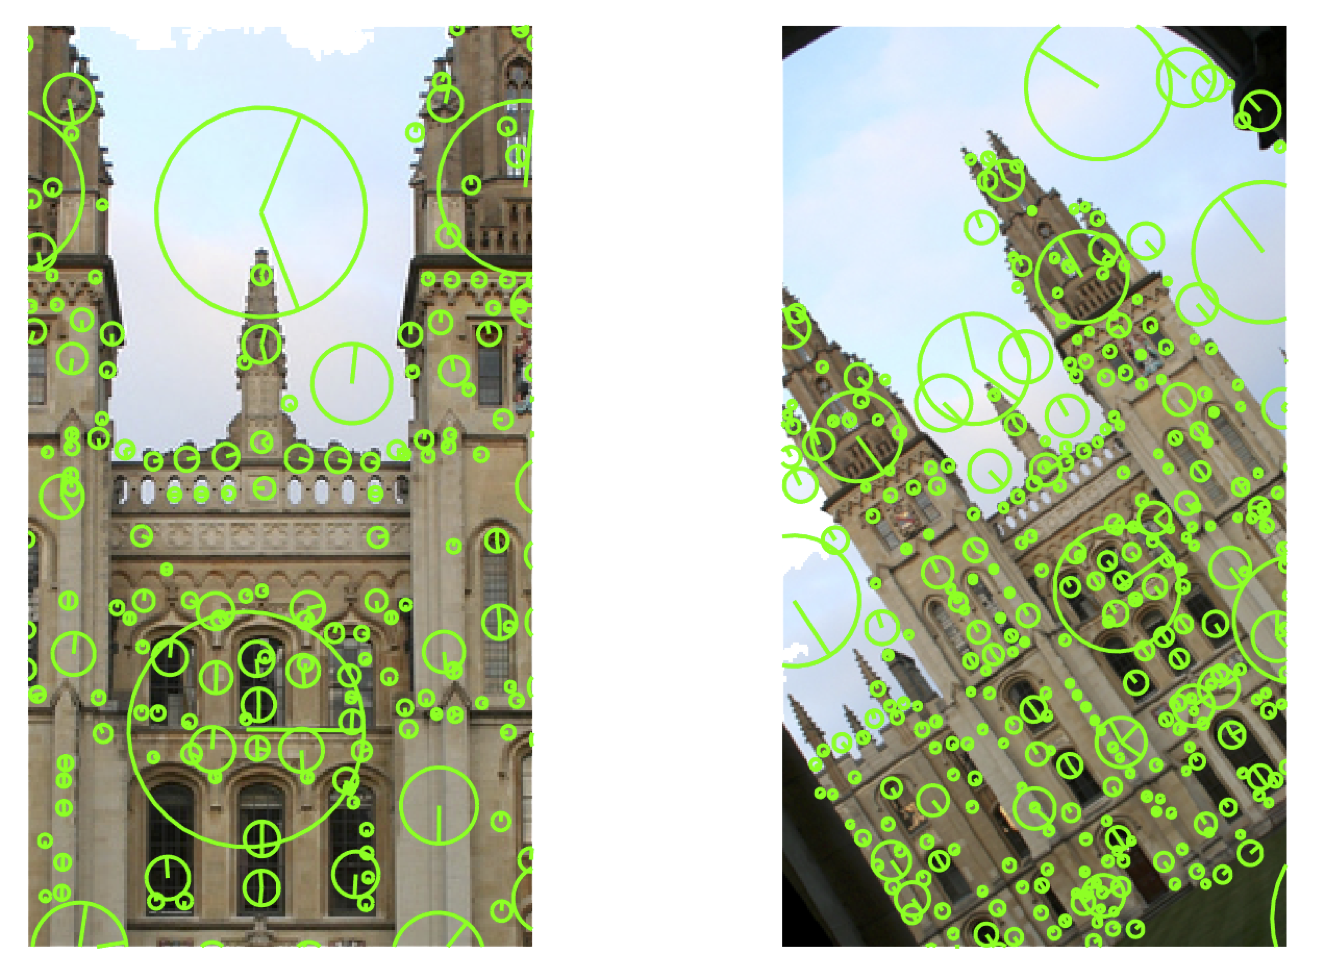
\includegraphics[height=8cm]{figures/siftDescriptor}
\end{center}
\caption{SIFT-descriptors visualized.}
\label{siftfeatures}
\end{figure}



\subsubsection{Approximate Nearest Neighbor}


\subsubsection{VLAD descriptor representation}
Vector of locally aggregated descriptors \(VLAD\) was developed in order to represent local descriptors so image searches could be done in a large scale with accuracy, efficiency and low memory consumption \cite{Jegou2010}.

ADC

IVFADC

k-means

component wide mass normalization

Square rooting

componentwise l-squared normalization

global l-squared normalization


\subsection{Receiver operating characteristic}
Receiver operating characteristic \(ROC\) graphs are good in visualizing and comparing classifier performance. In essence we are comparing three classifiers. ''A classifier is a mapping from instances to predicted classes'' \cite{Fawcett2006}. In our case the image is classified correctly by the classification system or it is not. This is a binary classification problem. The confusion matrix can be found in fig. \ref{figconfusion}. To compare the dct-, and simple perceptual hash classifiers to large scale image retrieval by SIFT features.

\begin{figure}[htb]
\begin{center}
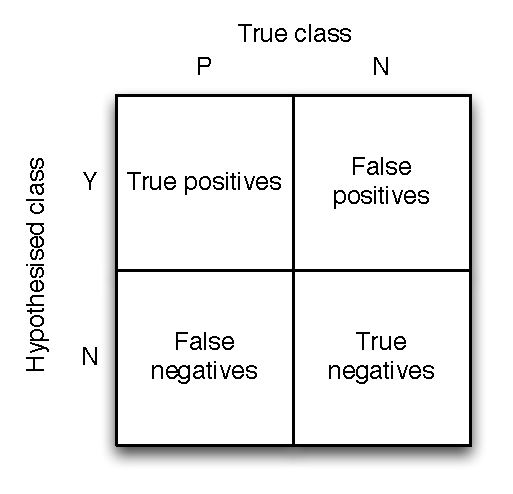
\includegraphics[height=8cm]{figures/confusion}
\end{center}
\caption{Confusion matrix for binary classification \cite{Fawcett2006}. }
\label{figconfusion}
\end{figure}

We adopt the notation from ROC paper by Tom Fawcett and use ${Y,N}$ for output from the classifier. For true classification we use ${p,n}$ for positive and negative respectively. In case of a true positive $p$ is classified correctly as $Y$. A false positive is a $p$ classified as a $N$. A false negative is $p$ classified as $N$ and true negative is $n$ classified as $N$. ROC space in fig. \ref{figrocspace} is made by plotting the $tp_{rate}$ vs. the $fp_{rate}$. The line from $(0,0)$ to $(1,1)$ represents classification by chance. Classifiers below this line do worse than luck itself. A discrete classifier outputs either $Y$ or $N$ or in our case image is found in the database or it is not. Discrete classifiers may be compared in ROC space like in fig.\ref{figrocspace} \cite{Fawcett2006}

\begin{figure}[htb]
\begin{center}
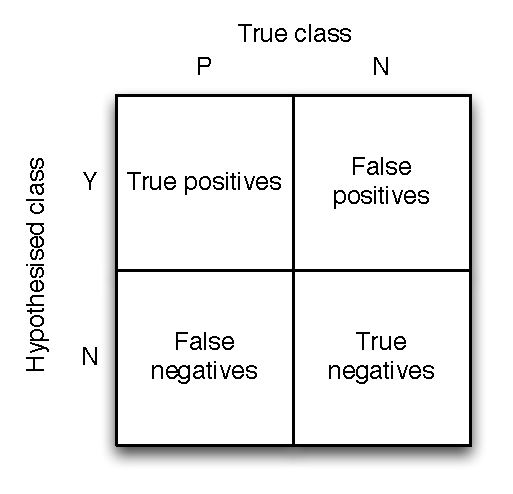
\includegraphics[height=8cm]{figures/ROC}
\end{center}
\caption{ROC space example with several discrete classifiers \cite{Fawcett2006}. }
\label{figrocspace}
\end{figure}


\begin{equation}
fp_{rate} = \frac{FP}{N}
\end{equation}
\begin{equation}
tp_{rate} = \frac{TP}{P}
\end{equation}
\begin{equation}
precision = \frac{TP}{TP + FP}
\end{equation}

\begin{equation}
recall = \frac{TP}{P}
\end{equation}

\begin{equation}
accuracy = \frac{TP + TN}{P + N}
\end{equation}

\subsection{Simulated classifier comparison}
\epigraph{Without data you're just another person with an opinion}{W. Edwards Deming}

To compare object instance recognition by SIFT features to perceptual hashing we will run simulations. We are faced with a binary classification problem. Receiver operating characteristics have been useful for visualizing classifier performance \cite{Fawcett2006}. We will construct ROC graphs for the simple hash, dct hash and large scale image retrieval with SIFT features.

To begin production implementation solving the near similar image matching problem with SIFT-features we need to know if the new solution is an improvement over the existing what we call the simple hash and a version DCT hash. A set of images is needed, as well as well as a modified set described in table \ref{modifiedimages} simulating scenarios typically encountered in duplicate image detection.

\def\arraystretch{1.5}
\begin{table}[htb]
\caption{Test image sets and motivations taken from the "Recognition of object instances practical" paintings set of images.}
\label{modifiedimages}
\begin{center}
\begin{tabular}{lp{0.5\linewidth}}
  Modification & Motivation \\
  \hline \hline
  53\% scale& Simulate responsive site case where image has a scaled duplicate. Choose prime percentage to avoid multiple of two to push scaler to produce uneven results.\\
  \hline
  83\% scale& Another scaled case \\
  \hline
  Shave 10px & Simulate cropping image by 10px or removing a border for example\\
  \hline
  10\% border & Adding a border to a known image \\
  \hline
  Rotate 10\% & User corrects the horizon of a photo \\
  \hline
  Normalize histogram & User normalizes the histogram of a photo\\
  \hline
  Saturate colors & User decides to modify the color palette of the image or photo\\
  \hline
  Not in database & Does the system classify images correctly as not in database?\\
\end{tabular}
\end{center}\end{table}

\def\arraystretch{1.5}
\begin{table}[htb]
\caption{True negatives dataset taken from the oxford images in "Recognition of object instances practical".}
\label{truenegatives}
\begin{center}
\begin{tabular}{lp{0.5\linewidth}}
  Modification & Motivation \\
  \hline \hline
  $n$ (true no) images  & Classify images correctly as $N$?\\
\end{tabular}
\end{center}\end{table}

Paintings dataset from the "Recognition of object instances practical" \cite{Vedaldi2012} of a total of 1708 images will be used due to ready scripts for the SIFT case.

An Imagemagick shell script generates manipulated duplicates. 53\% and 83\% scales simulate multiple scales of the same image. Photo straightening is simulated by a 10\% rotation. For color manipulation so we will saturate the image by 50\%. Histogram normalization is quite a common operation, so we will use a normalized version of the image to try to find matches.

To simulate image cropping, we crop from all sides by $10px$. Adding a border is simulated by making duplicates with a 10px border.

To test for images not in the set we will pick 1708 images from the ''Object instance recognition practical'' Oxford dataset and run those images against the paintings set. This will look for a $fp_{rate}$ rate with images that are not in the dataset.

Since we do not know how hamming distance affects classifier performance, we will run all sets for hamming distances 0,4,8 \& 12 to tune the hamming distance.

\subsection{System for near duplicate detection by local features}

\subsection{Edge cases}
Images smaller than 32px wide or high are ignored by the simple hash and dct hash algorithms. Annotating small images is counterproductive so they are ignored.

\clearpage

\section{Results}
Modified image sets in tables \ref{modifiedimages} and \ref{truenegatives} were run against all three classifiers, the simple hash, the dct hash and SIFT-classifier. SIFT-classifier outperforms the perceptual hashes in all categories except the simple hash for 53\% scale fig. \ref{tptotal}. The only miss for the SIFT-matcher is a duplicate image in the paintings dataset. SIFT outperforms the perceptual hashes for FP for all test sets in fig. \ref{fpTotal}.

For the $TN$ test set the SIFT-classifier performed the worst returning all false positives instead of misses. This was due to not setting a cutoff score. If returned matches from a search score less than this cutoff score, the image should be classified as a $TN$. The max score from the $TN$-set was 19 (fig. \ref{sifttnscores}). In order to determine optimum cutoff, we simulate setting the cutoff score from 1 to 19 and run the simulations for each cutoff score.



\begin{figure}[htb]
\begin{center}
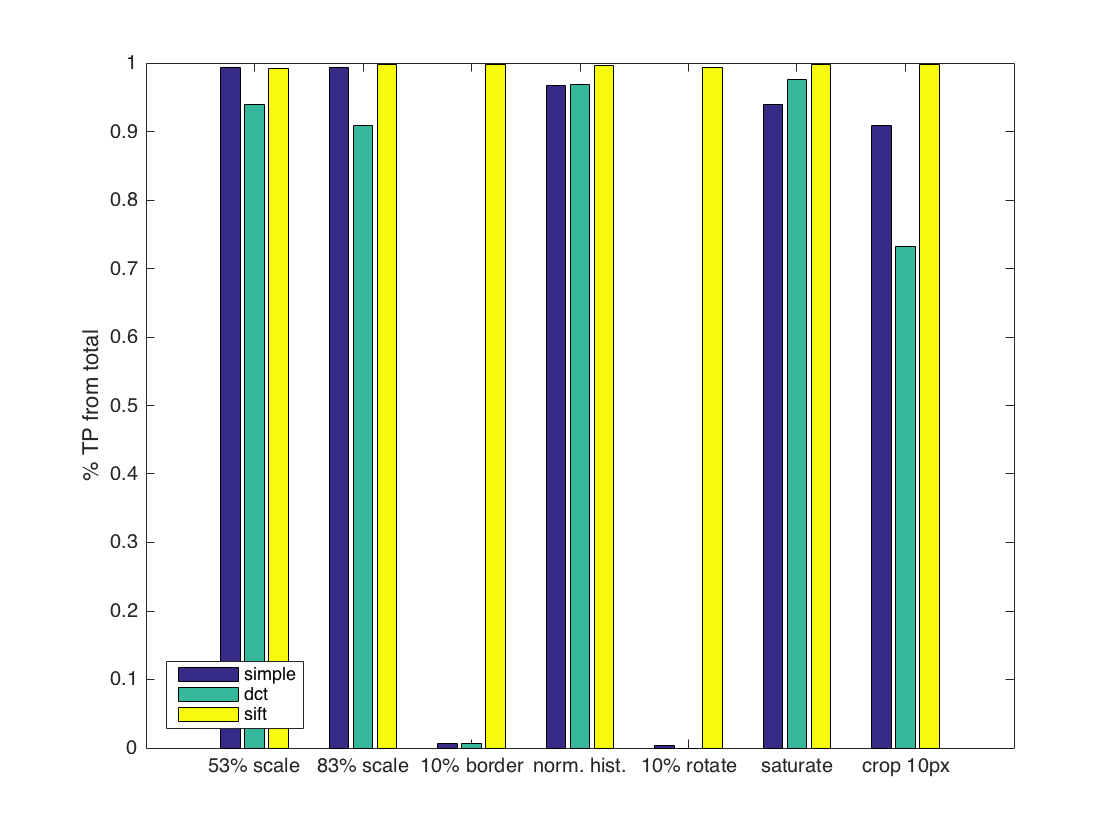
\includegraphics[height=8cm]{figures/tpBar}
\end{center}
\caption{ $TP$ for near duplicate modifications in table \ref{modifiedimages} }
\label{tptotal}
\end{figure}


\begin{figure}[htb]
\begin{center}
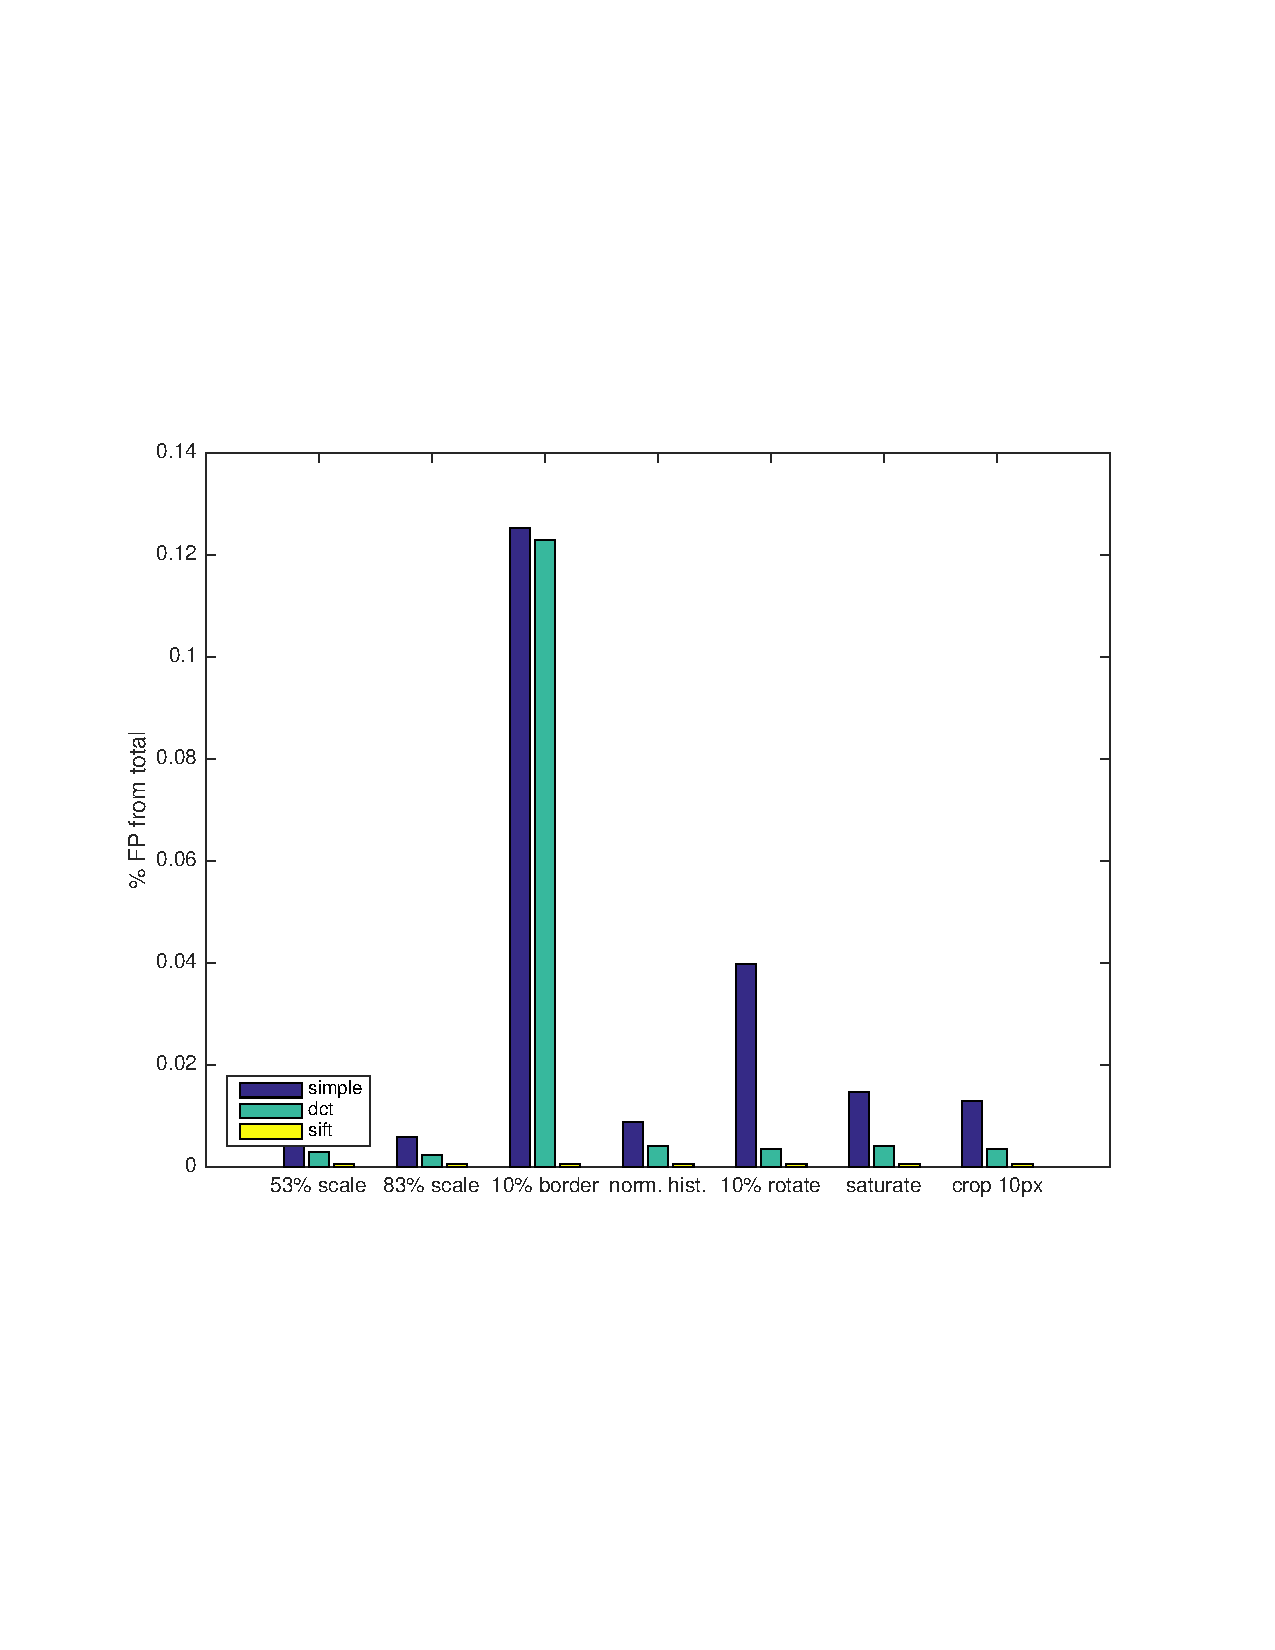
\includegraphics[height=8cm]{figures/fpBar}
\end{center}
\caption{ $FP$ for near duplicate modifications in table \ref{modifiedimages} }
\label{fptotal}
\end{figure}


\begin{figure}[htb]
\begin{center}
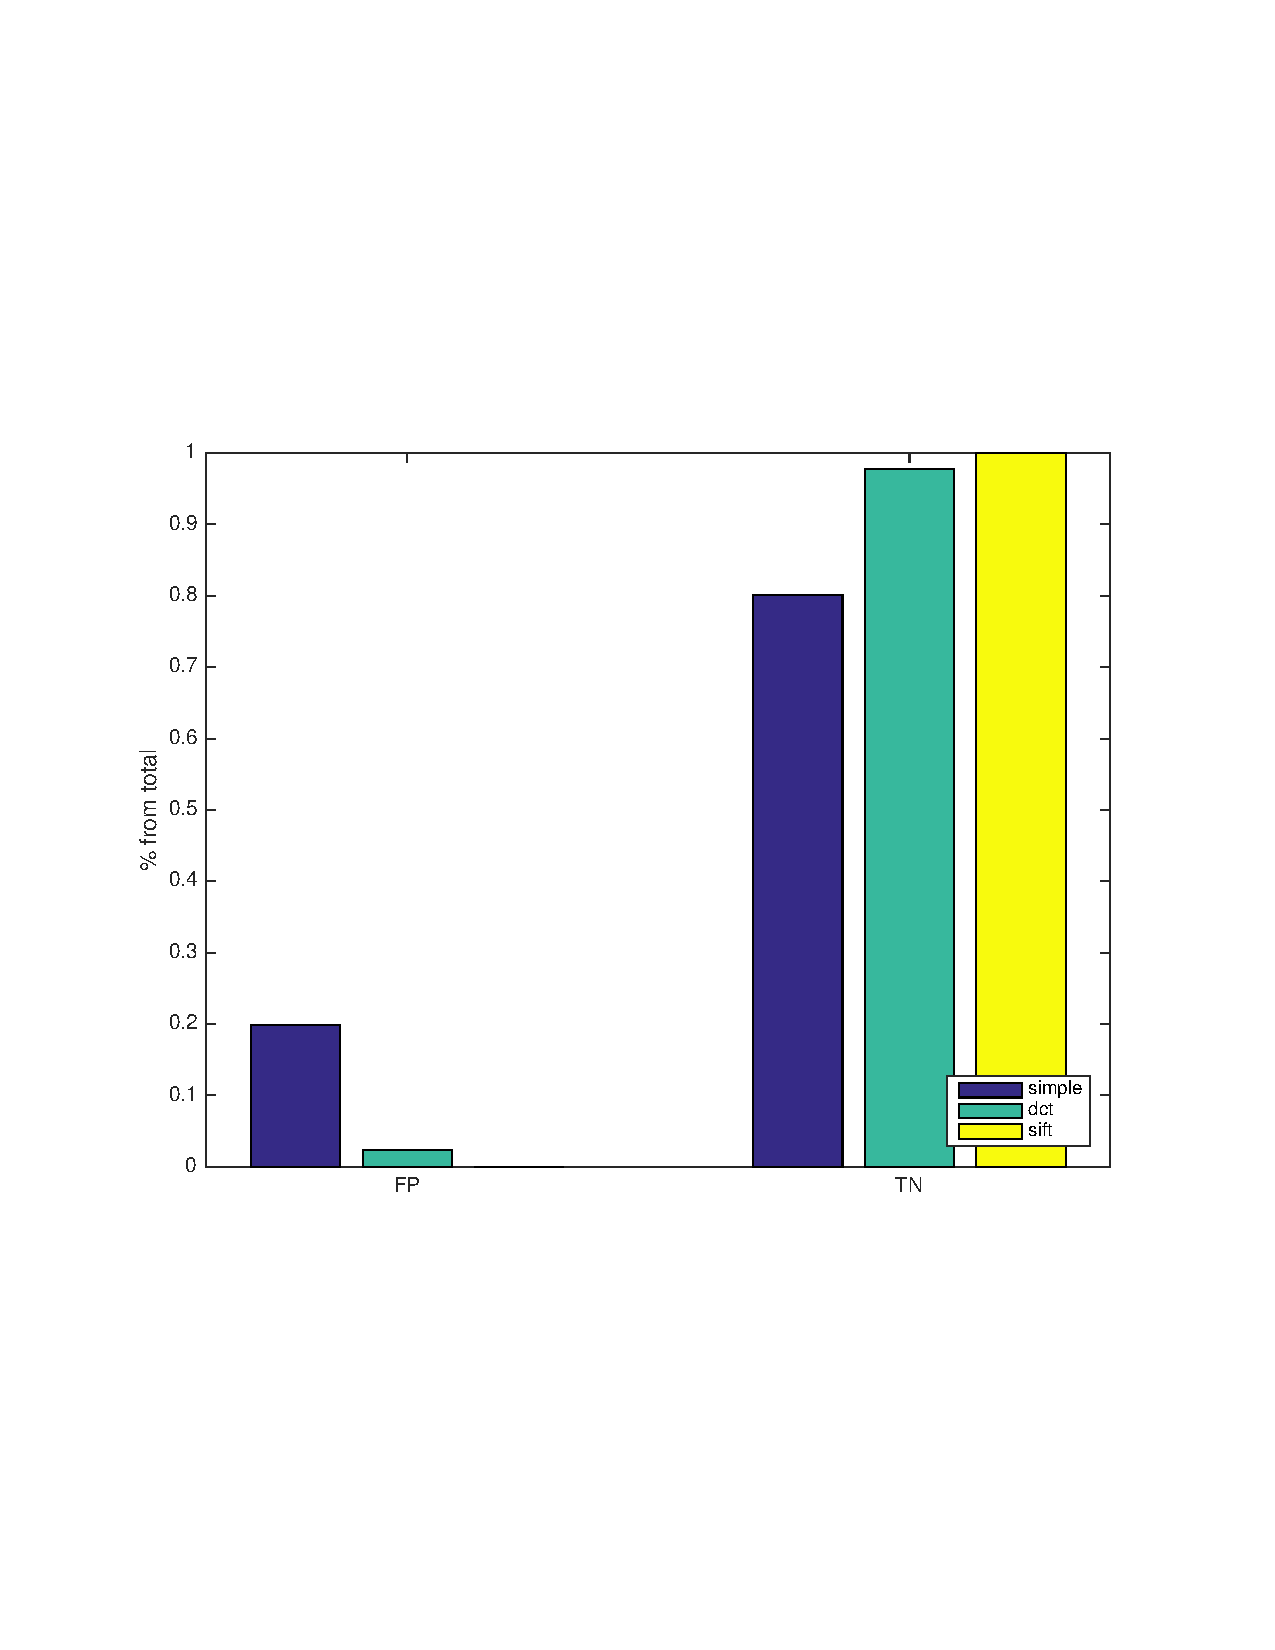
\includegraphics[height=8cm]{figures/tnBar}
\end{center}
\caption{ $TN$ for near duplicate modifications in table \ref{tnimages} }
\label{tntotal}
\end{figure}

\begin{figure}[htb]
\begin{center}
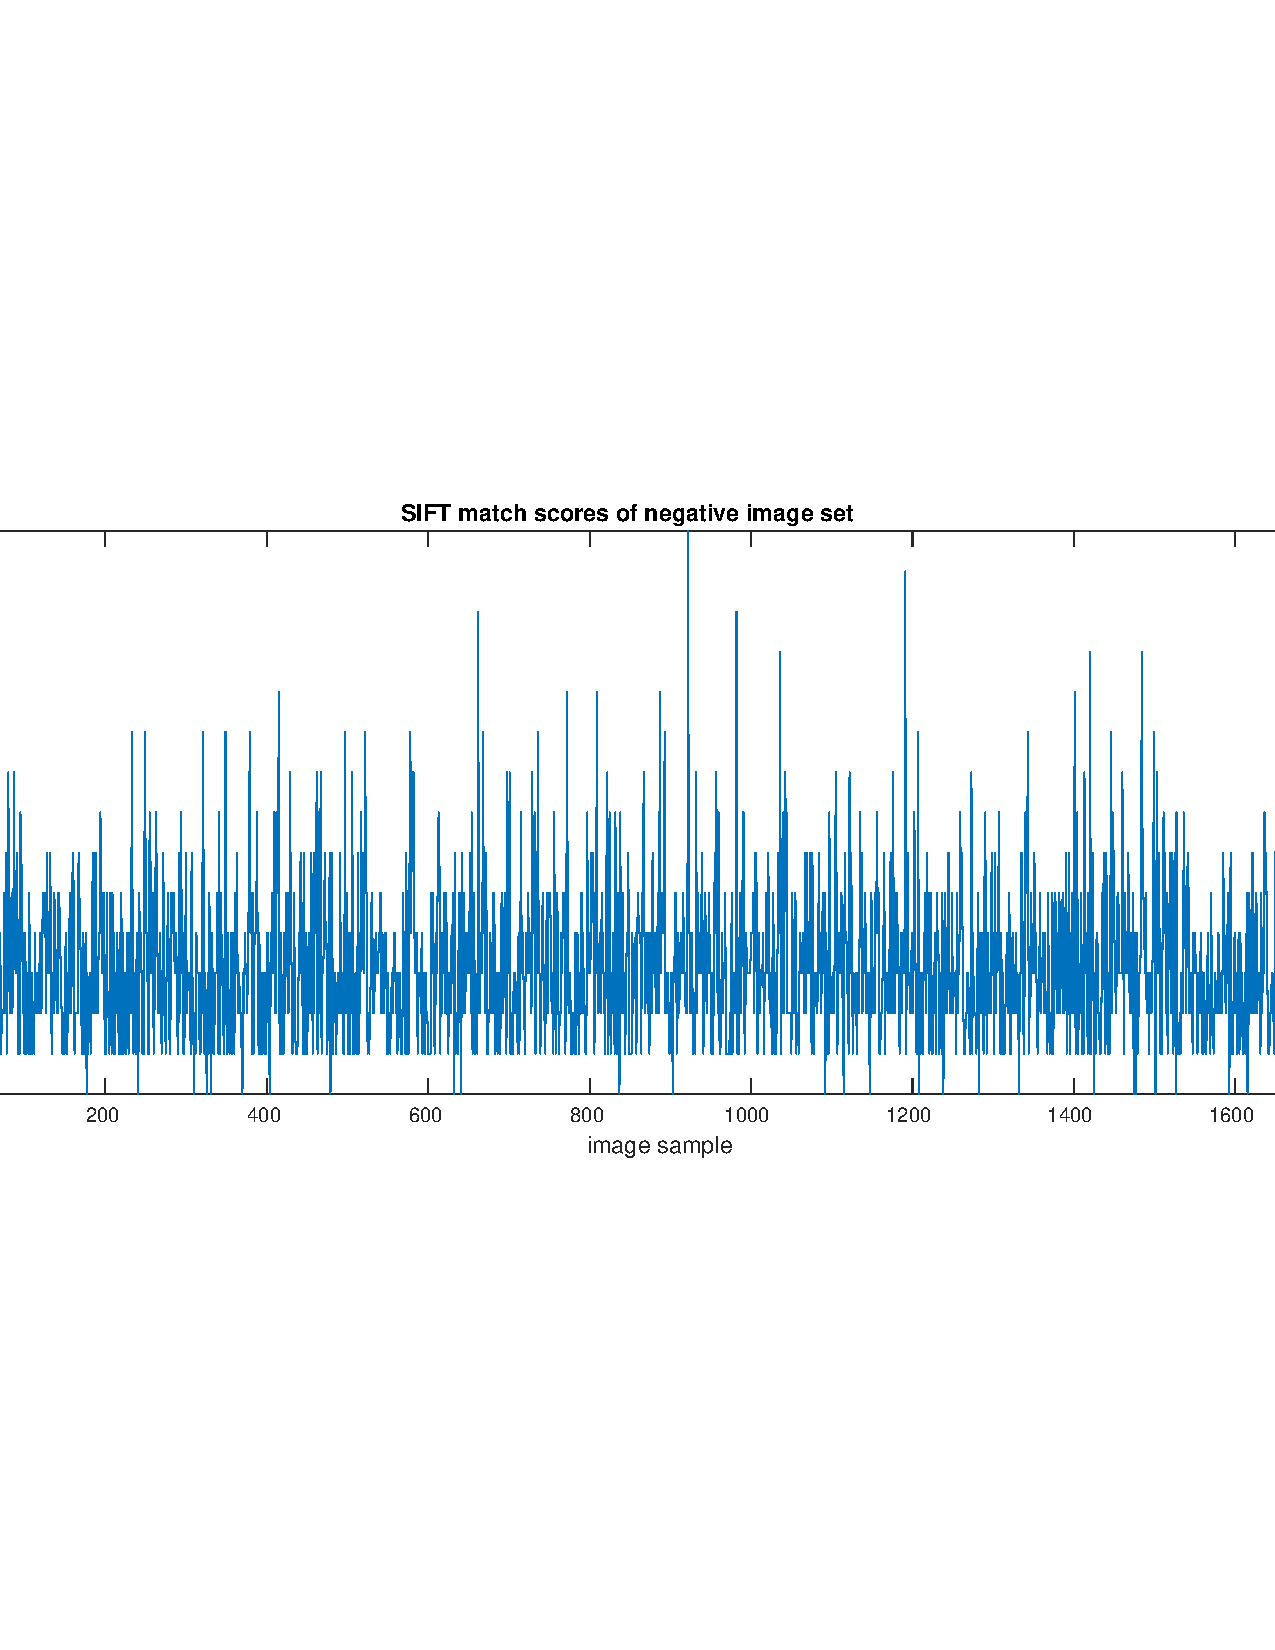
\includegraphics[height=8cm]{figures/cutoff}
\end{center}
\caption{ $TN$ image set max scores returned for images not in database \ref{tnimages} }
\label{sifttnscores}
\end{figure}




\subsection{Simple hash}

\subsection{DCT Hash}
The $ROC$ of a dct hash based matcher depends on the chosen hamming distance tolerance. The effect on setting hamming distance tolerance on dct hash matcher can be seen in fig. \ref{dcttotalaccuracy}

\begin{figure}[htb]
\begin{center}
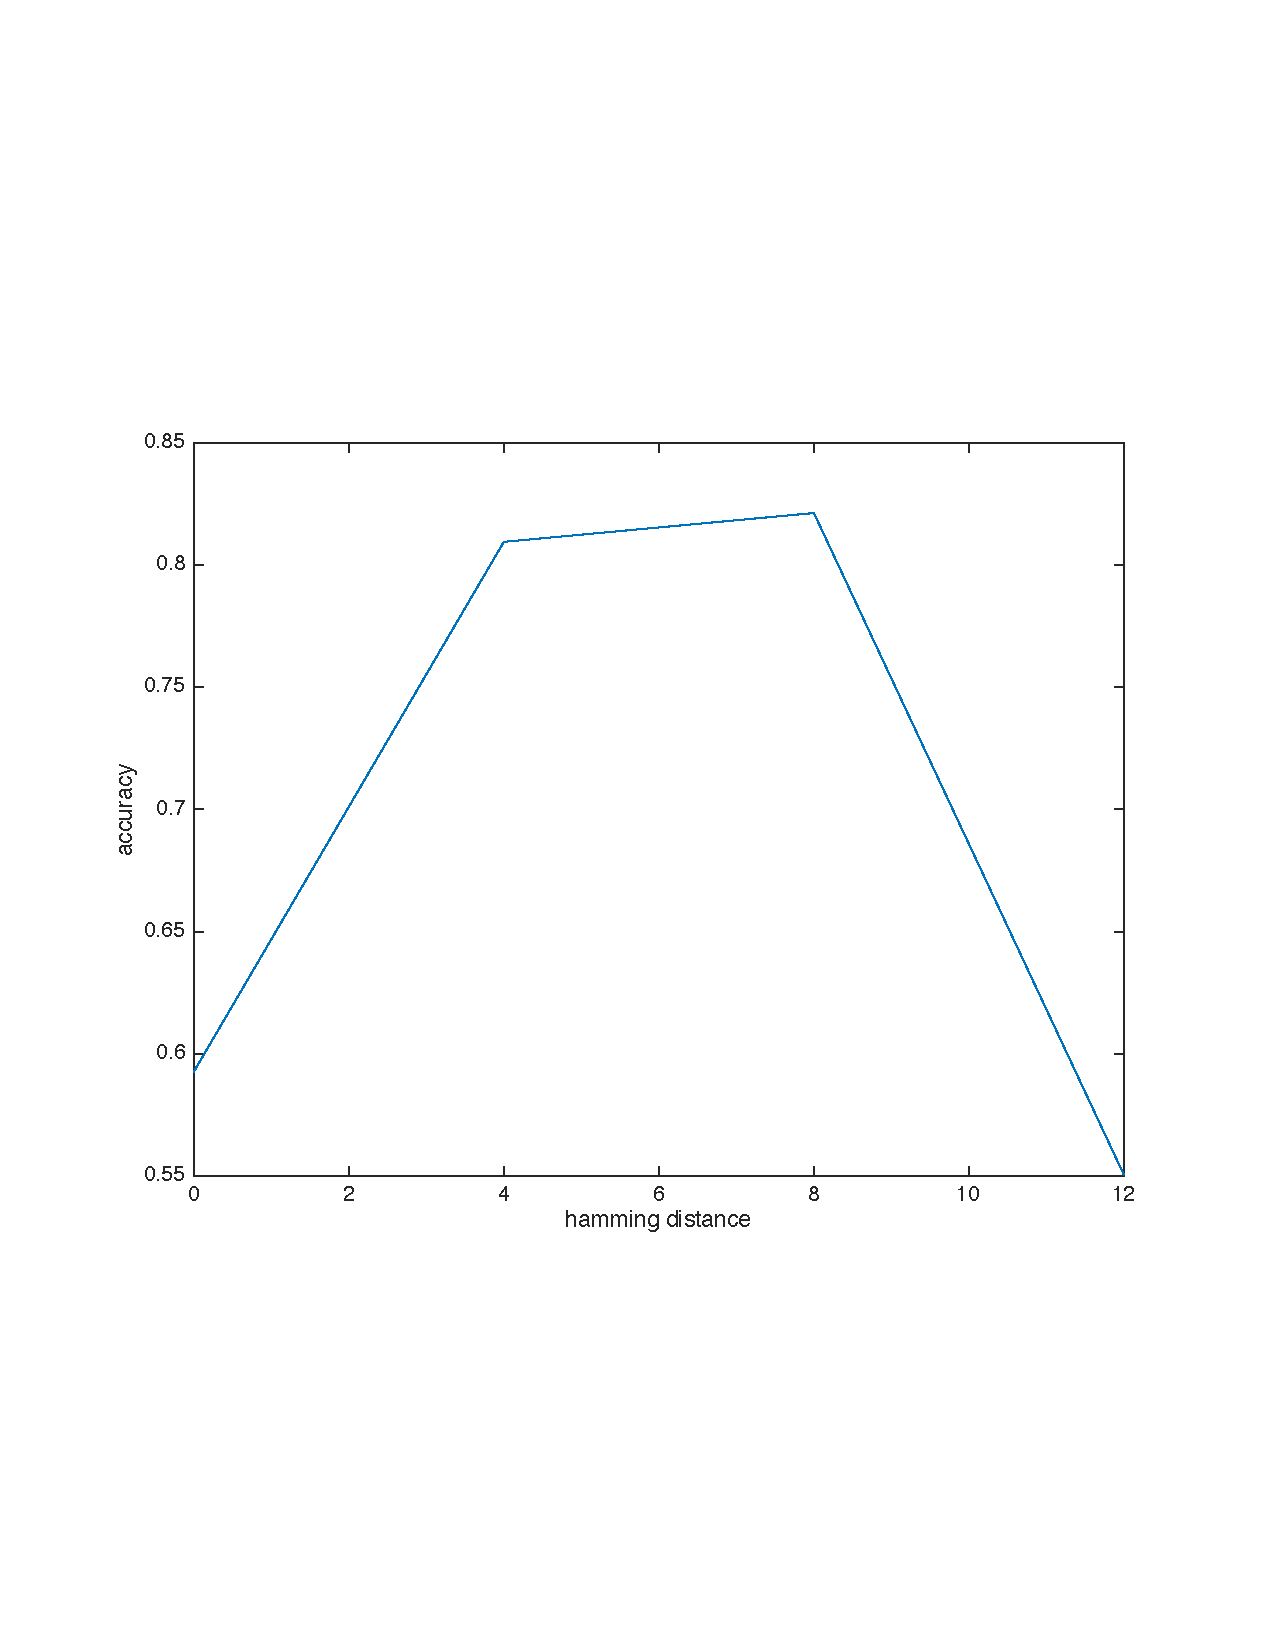
\includegraphics[height=8cm]{figures/dctTotalAccuracy}
\end{center}
\caption{ Effect of Hamming distance tolerance on total accuracy of DCT classifier. }
\label{dcttotalaccuracy}
\end{figure}

\begin{figure}[htb]
\begin{center}
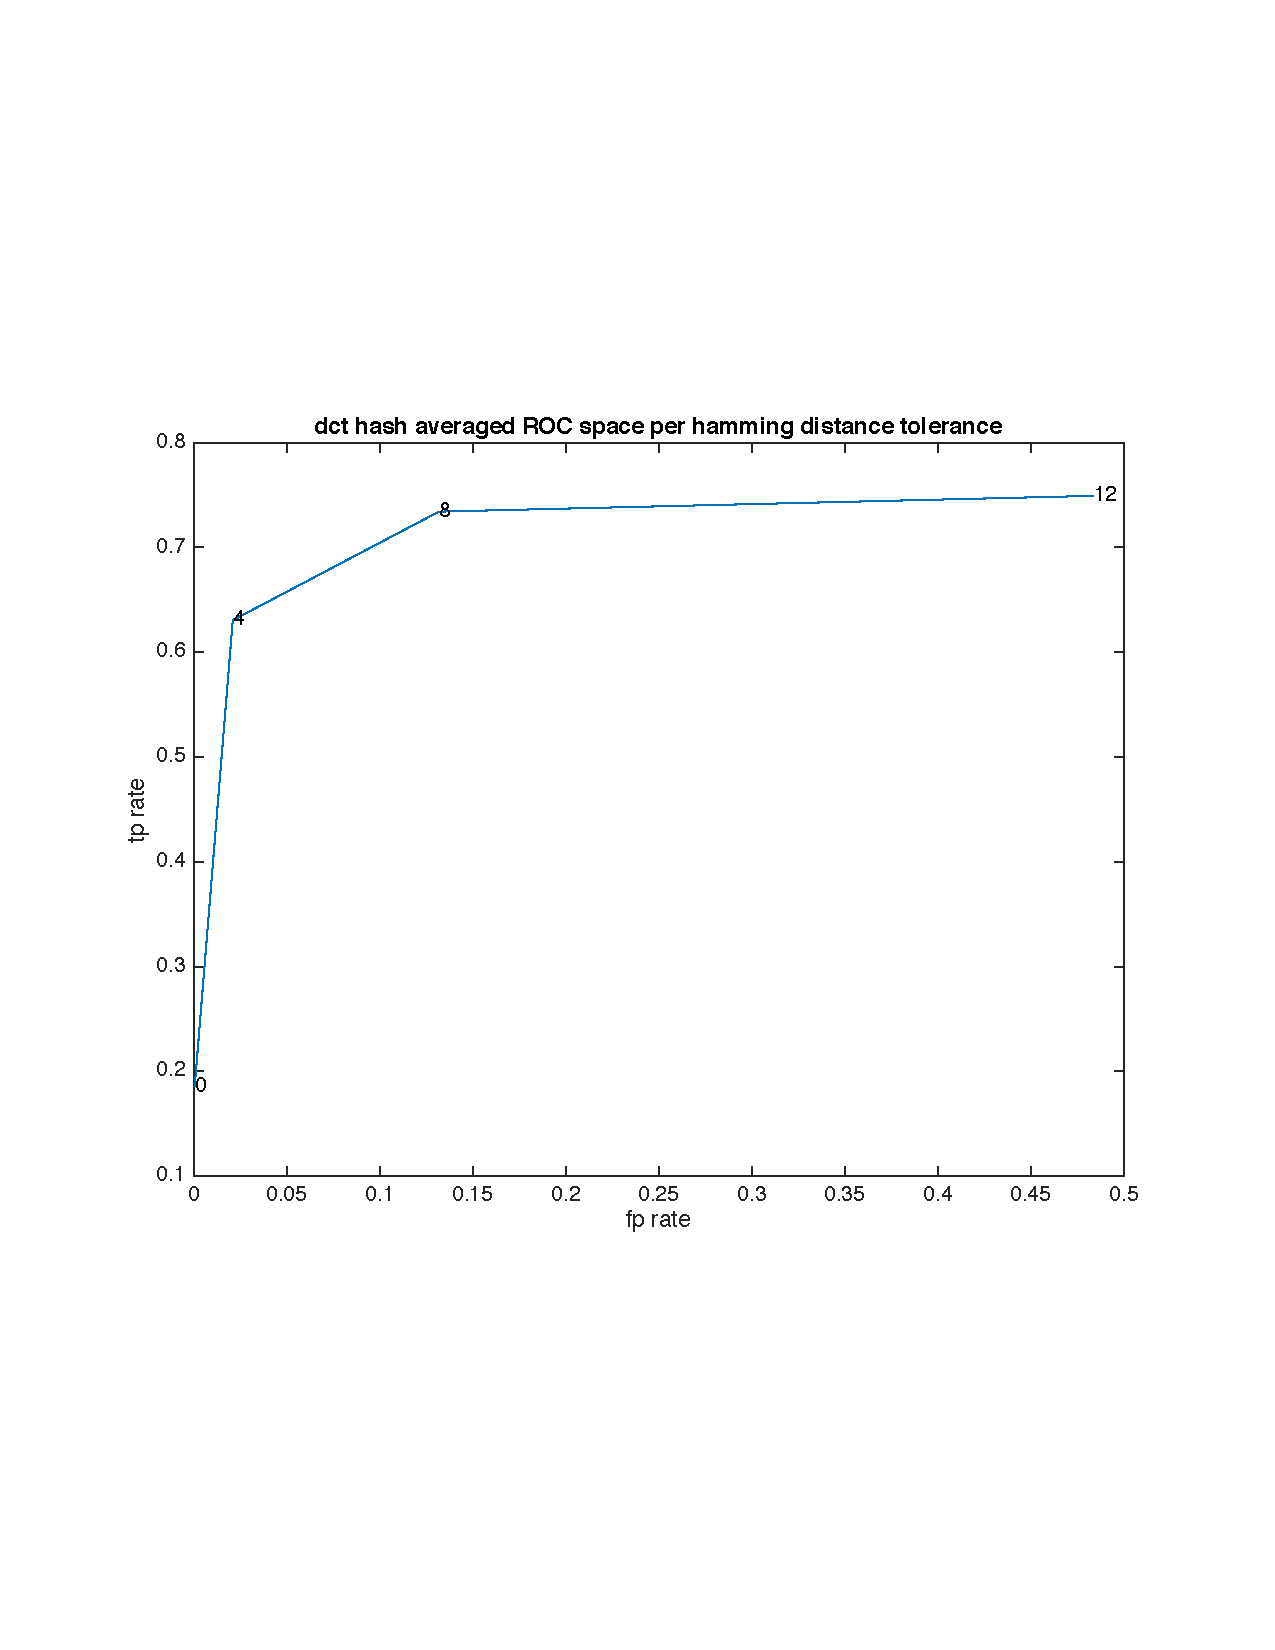
\includegraphics[height=8cm]{figures/dctTotalROC}
\end{center}
\caption{ ROC space per hamming distance tolerance based on averaging results on all data. }
\label{dcttotalaccuracy}
\end{figure}

\subsubsection{Hamming distance}

\subsection{Object instance detection by SIFT features}

\subsubsection{Cutoff $C_{s}$}
The search by $SIFT$-features will always return the highest scoring image even if the case of a $fp$. A sane $fp_{rate}$ (close to zero) can be achieved by choosing a cutoff score so that as many as possible of the sets in table \ref{modifiedimages}, and keep true misses to a minimum. We run the sets and plot the scores of matches from each set and find a score such that $tp_{rate}$ is maximized and $fp_{rate}$ is minimized.

Fig. \ref{figcutoffrocspace} shows $SIFT$-classifier performance degrade as $C_{s}->0$. From fig.\ref{figcutoff} we can see the $fn_{count}$ increase linearly as cutoff increases where as the $fp_{count}$ decreases logarithmically as cutoff goes to 19. Plotting the accuracy (eq. \ref{accuracy}) of a the SIFT classifier per $C_{s}$ over data from runs of images in table \ref{modifiedimages} up to

\begin{equation}\label{maxtnscore}
max(score_{tndata}) = 19
\end{equation}

Vertical and horizontal flips are excluded as we do not expect our classifiers to perform well on those. From the test in table \ref{truenegatives}. From fig.\ref{figcutoff} accuracy section we can deduce that the highest accuracy for this data can be achieved by setting $C_{s} = max(score_{tn}) = 19$.

\begin{equation} \label{accuracy}
ACC = \frac{TP +TN}{TP + FP + TN + FN}
\end{equation}

\begin{figure}[htb]
\begin{center}
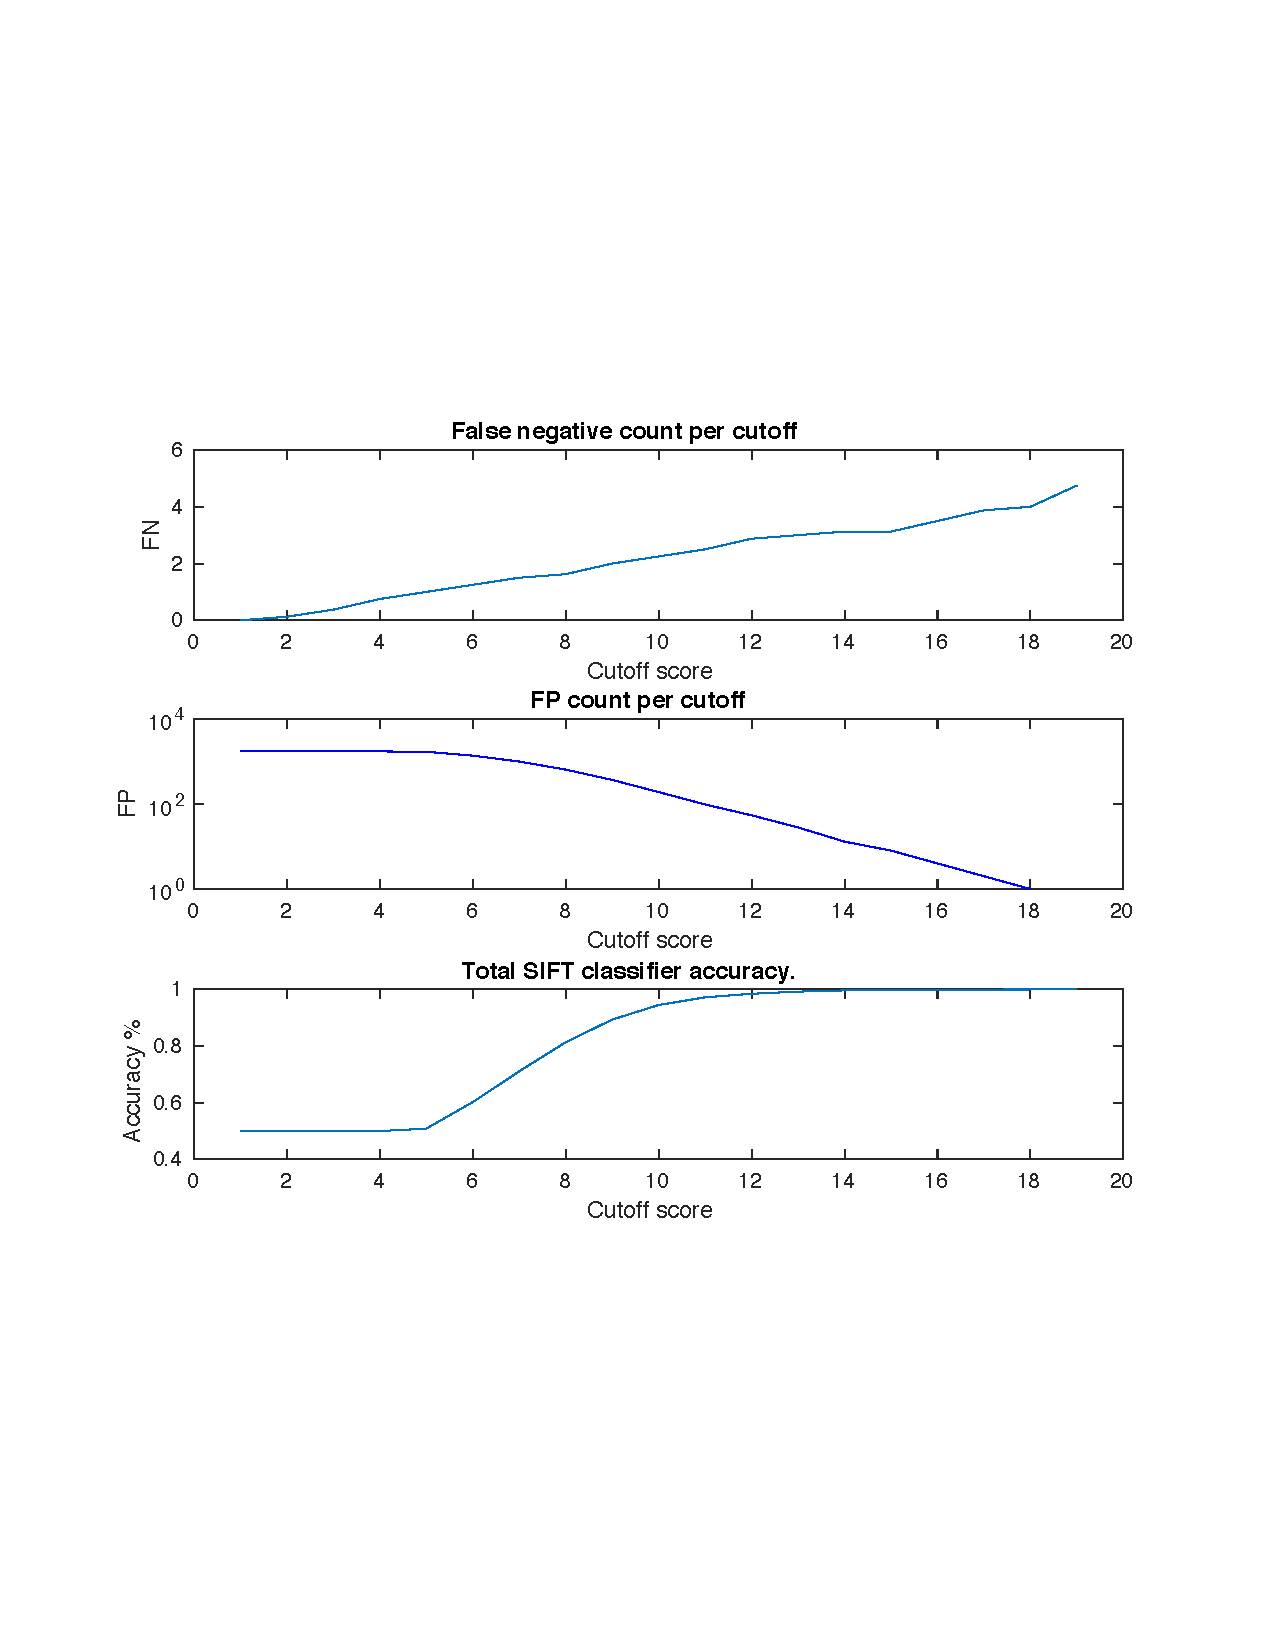
\includegraphics[height=8cm]{figures/SIFTCountROC}
\end{center}
\caption{ Effects of cutoff on SIFT performance. }
\label{figcutoff}
\end{figure}

\begin{figure}[htb]
\begin{center}
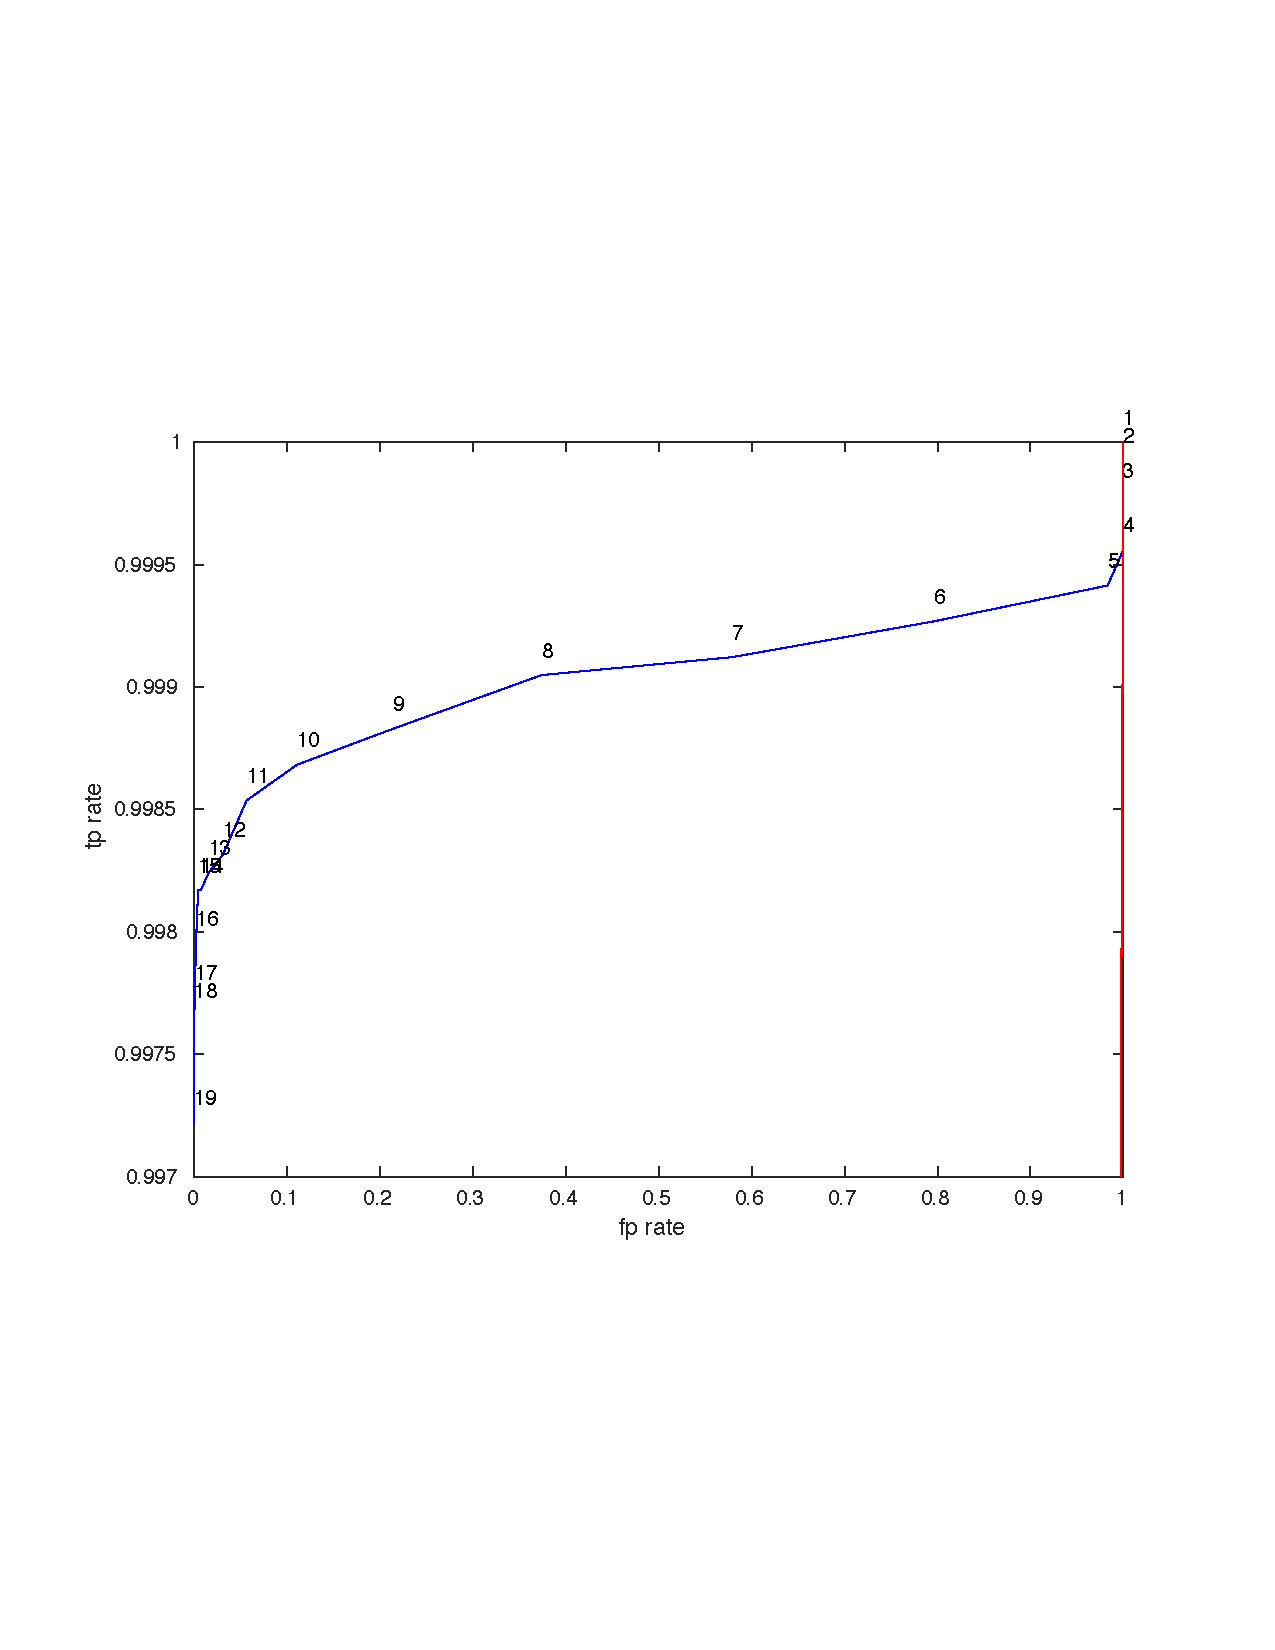
\includegraphics[height=8cm]{figures/SIFTROCperCutoff}
\end{center}
\caption{ ROC Space per SIFT classifier cutoff. }
\label{figcutoffrocspace}
\end{figure}



\subsection{Simulated classifier comparison}
All classifiers in ROC space.

The optimum hamming distance for the classifier using simple hash seems to be 4.
The optimum hamming distance to use with a dct hash classifier seems to be 4.

A table of all the tp and fp rates.
A table with all the numbers from the ROC section.

Put all classifiers in ROC space for all cases.

roc graph over all cases in small multiples

\subsection{System for near duplicate detection by local features}


\clearpage

\section{Discussion}
Any conclusions from the ROC graphs. What recommendation to make? What to take a look at.



\clearpage
%% L\"ahdeluettelo
%%
%% \phantomsection varmistaa, ett\"a hyperref-paketti latoo hypertekstilinkit
%% oikein.
%%
%% The \phantomsection command is nessesary for hyperref to jump to the
%% correct page, in other words it puts a hyper marker on the page.

\phantomsection
\addcontentsline{toc}{section}{\refname}
%\addcontentsline{toc}{section}{References}
\bibliographystyle{plain}
\bibliography{sources}{}

%% Appendices
%% Liitteet
\clearpage

\thesisappendix

\section{Esimerkki liitteest\"a\label{LiiteA}}

Liitteet eiv\"at ole opinn\"aytteen kannalta v\"altt\"am\"att\"omi\"a ja
opinn\"aytteen tekij\"an on
kirjoittamaan ryhtyess\"a\"an hyv\"a ajatella p\"arj\"a\"av\"ans\"a ilman liitteit\"a.
Kokemattomat kirjoittajat, jotka ovat huolissaan
tekstiosan pituudesta, paisuttavat turhan
helposti liitteit\"a pit\"a\"akseen tekstiosan pituuden annetuissa rajoissa.
T\"all\"a tavalla ei synny hyv\"a\"a opinn\"aytett\"a.

Liite on itsen\"ainen kokonaisuus, vaikka se t\"aydent\"a\"akin tekstiosaa.
Liite ei siten ole pelkk\"a listaus, kuva tai taulukko, vaan
liitteess\"a selitet\"a\"an aina sis\"all\"on laatu ja tarkoitus.

Liitteeseen voi laittaa esimerkiksi listauksia. Alla on
listausesimerkki t\"am\"an liitteen luomisesta.

%% Verbatim-ymp\"arist\"o ei muotoile tai tavuta teksti\"a. Fontti on monospace.
%% Verbatim-ymp\"arist\"on sis\"all\"a annettuja komentoja ei LaTeX k\"asittele.
%% Vasta \end{verbatim}-komennon j\"alkeen jatketaan k\"asittely\"a.
\begin{verbatim}
	\clearpage
	\appendix
	\addcontentsline{toc}{section}{Liite A}
	\section*{Liite A}
	...
	\thispagestyle{empty}
	...
	teksti\"a
	...
	\clearpage
\end{verbatim}

Kaavojen numerointi muodostaa liitteiss\"a oman kokonaisuutensa:
\begin{eqnarray}
d \wedge A  &=& F, \label{liitekaava1}\\
d \wedge F  &=& 0. \label{liitekaava2}
\end{eqnarray}


\clearpage
\section{Toinen esimerkki liitteest\"a\label{LiiteB}}

%% Liitteiden kaavat, taulukot ja kuvat numeroidaan omana kokonaisuutenaan
%%
%% Equations, tables and figures have their own numbering in Appendices
%\renewcommand{\theequation}{B\arabic{equation}}
%\setcounter{equation}{0}
%\renewcommand{\thefigure}{B\arabic{figure}}
%\setcounter{figure}{0}
%\renewcommand{\thetable}{B\arabic{table}}
%\setcounter{table}{0}

Liitteiss\"a voi my\"os olla kuvia, jotka
eiv\"at sovi leip\"atekstin joukkoon:
%% Ymp\"arist\"on figure parametrit htb pakottavat
%% kuvan t\"ah\"an, eik\"a LaTeX yrit\"a siirrell\"a niit\"a
%% hyv\"aksi katsomaansa paikkaan.
%% Ymp\"arist\"o\"a center voi k\"aytt\"a\"a \centering-
%% komennon sijaan
%%
%% Example of a figure, note the use of htb parameters which force
%% the figure to be inserted here
\begin{figure}[htb]
\begin{center}

\includegraphics[height=8cm]{kuva2}
\end{center}
\caption{Kuvateksti, jossa on liitteen numerointi}
\label{liitekuva}
\end{figure}
%%
Liitteiden taulukoiden numerointi on kuvien ja kaavojen kaltainen:
\begin{table}[htb]
\caption{Taulukon kuvateksti.}
\label{liitetaulukko}
\begin{center}
\fbox{
\begin{tabular}{lp{0.5\linewidth}}
9.00--9.55  & K\"aytett\"avyystestauksen tiedotustilaisuus (osanottajat
ovat saaneet s\"ahk\"opostitse valmistautumisteht\"av\"at, joten tiedotustilaisuus
voidaan pit\"a\"a lyhyen\"a).\\
9.55--10.00 & Testausalueelle siirtyminen
\end{tabular}}
\end{center}
\end{table}
Kaavojen numerointi muodostaa liitteiss\"a oman kokonaisuutensa:
\begin{eqnarray}
T_{ik} &=& -p g_{ik} + w u_i u_k + \tau_{ik},  \label{liitekaava3} \\
n_i    &=& n u_i + v_i.                      \label{liitekaava4}
\end{eqnarray}

\end{document}
